\section{Specifications}
\label{sec:specs}
\newcounter{SpecID}

\subsection{Arena}
\refstepcounter{SpecID}
\label{spec:arena}

\begin{enumerate}
  \item The arena floor is an \SI{9}{m} $\times$ \SI{9}{m} rectangle. The
        tolerance of these two dimensions is $\pm$ \SI{250}{mm}.
  \item The floor of the arena is carpeted.
  \item The layout of the arena is given in Figure~\ref{fig:arena}. This
        figure is to scale.
  \item The outer walls of the arena are at least \SI{600}{mm} high, and the
        interior surface is white plastic-coated hardboard.
  \item Each of scoring zones is \SI{2.4}{m} $\times$ \SI{2.4}{m} $\pm$ \SI{100}{mm},
        resulting in a total size of \SI{4.8}{m} $\times$ \SI{4.8}{m} $\pm$ \SI{200}{mm}
        for the four scoring zones.
  \item Scoring zones are bounded by metallic tape around the perimeter
        and internal boundaries. The inside edge of the tape marks the outside
        edge of the scoring zone.
  \item The raised area in the centre of the arena is \SI{2.4}{m} $\times$ \SI{2.4}{m} $\pm$ \SI{100}{mm},
        with a height of \SI{180}{mm} $\pm$ \SI{10}{mm}.
  \item At the cardinal points of the arena are \SI{1.2}{m} $\times$ \SI{1.2}{m} $\pm$ \SI{100}{mm} walls,
        raised at least \SI{180}{mm} $\pm$ \SI{10}{mm}.
  \item Scoring zones for teams are offset 90\degree{} anti-clockwise, such
        that a team isn't directly in front of their own scoring zone.
  \item Each robot will be assigned a corner at the start of every match to indicate its starting area.
        Corner starting areas are \SI{1000}{mm} $\pm$ \SI{20}{mm} square and will be marked by tape.
\end{enumerate}

\begin{figure}
  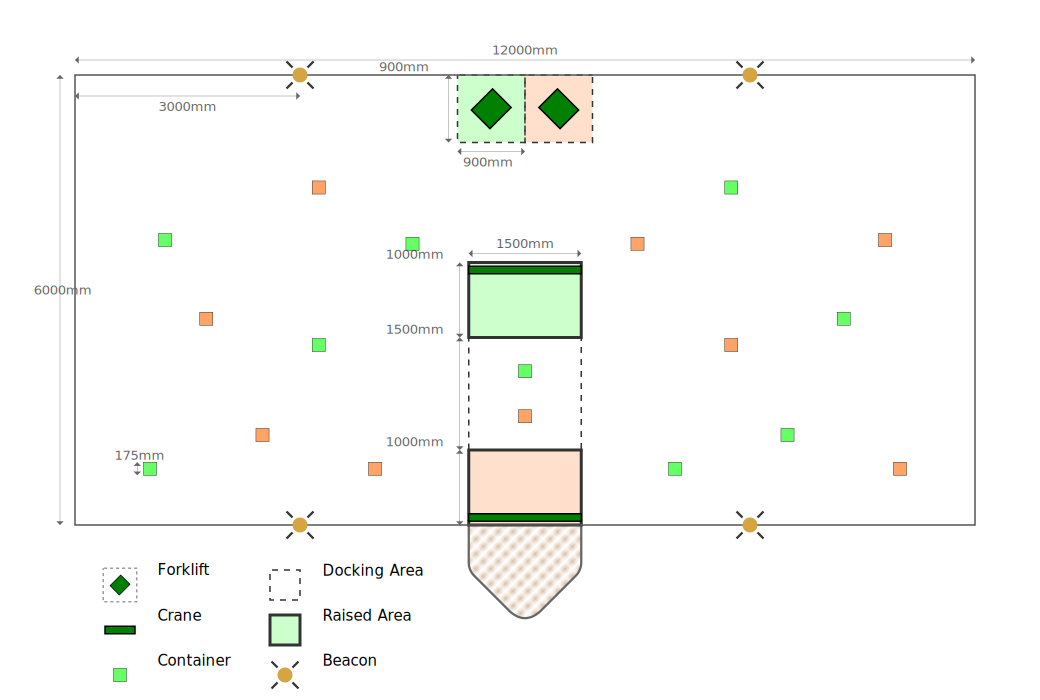
\includegraphics[scale=0.58]{fig-arena.pdf}
  \caption{Layout zones and tokens in the arena.}
  \label{fig:arena}
\end{figure}

\subsection{Tokens}
\refstepcounter{SpecID}
\label{spec:tokens}

\begin{enumerate}
  \item The tokens are cuboids with side length \SI{250}{mm} $\pm$ \SI{10}{mm}.
  \item 4 tokens are placed in each quadrant of the arena, in a rotationally
        symmetrical pattern, as indicated in Figure~\ref{fig:arena}.
  \item Robots will start with 1 token equidistant between the edge of their
        starting area and the nearest scoring zones.
  \item The starting positions of the tokens will be at least \SI{500}{mm} from the
        scoring zones or arena walls.
  \item Each face of each token is bordered by \SI{10}{mm} $\pm$ \SI{2}{mm} of
        copper conductive tape
\end{enumerate}
